%----------------------------------------------------------------------------------------
%	Appendices
%----------------------------------------------------------------------------------------

\part{Appendices}

\chapter{Hardware Topologies}

Appendix A contains circuit diagrams relating to hardware sensing and processing topologies. All component designators are arbitrary except R1, R2, R3, and R4 which represent the four load cells. Further, + and - are the positive and negative relationship strain gauges inside the load cells.

\begin{figure}[!ht]
	\centering
	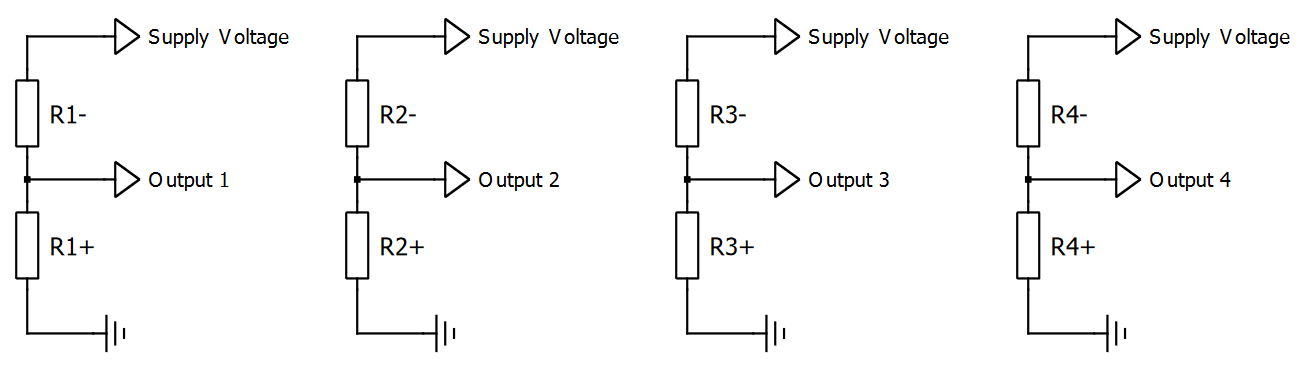
\includegraphics[scale=0.5]{hw-sensing-1.png}
	\caption{Individual load cell sensing topology.}
	\label{fig:sense-1}
\end{figure}

\begin{figure}[!ht]
	\centering
	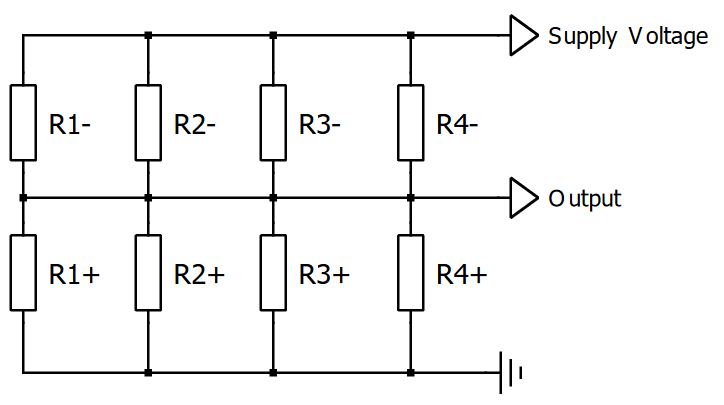
\includegraphics[scale=0.45]{hw-sensing-2.png}
	\caption{Parallel load cell sensing topology.}
	\label{fig:sense-2}
\end{figure}

\begin{figure}[!ht]
	\centering
	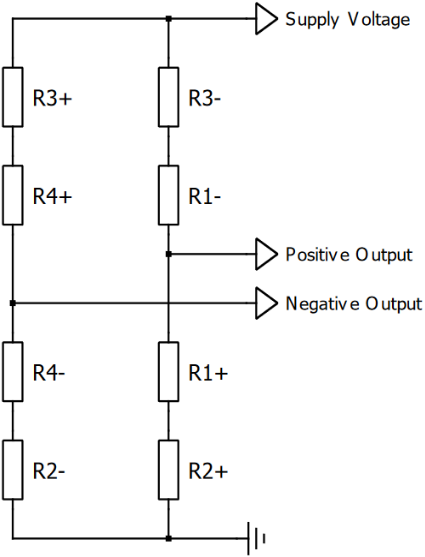
\includegraphics[scale=0.5]{hw-sensing-3.png}
	\caption{a) One load cell Wheatstone bridge b) Four load cell Wheatstone Bridge.}
	\label{fig:sense-3}
\end{figure}

\begin{figure}[!ht]
	\centering
	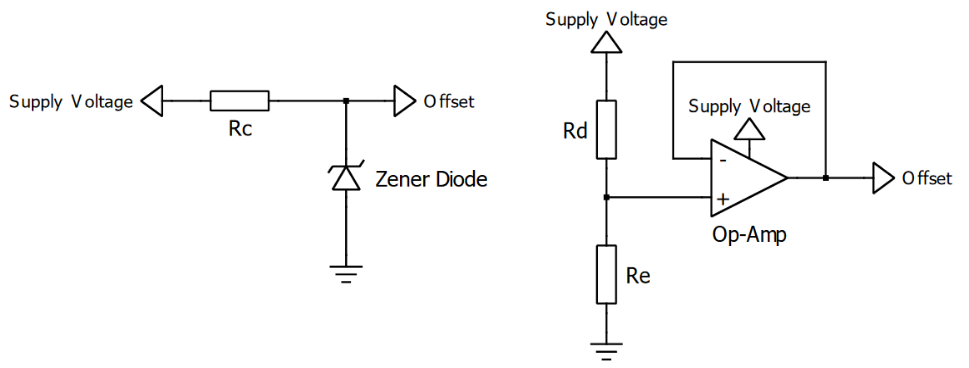
\includegraphics[scale=0.6]{hw-offset.png}
	\caption{a) Zener regulator b) Voltage divider with buffer.}
	\label{fig:offset}
\end{figure}

\begin{figure}[!ht]
	\centering
	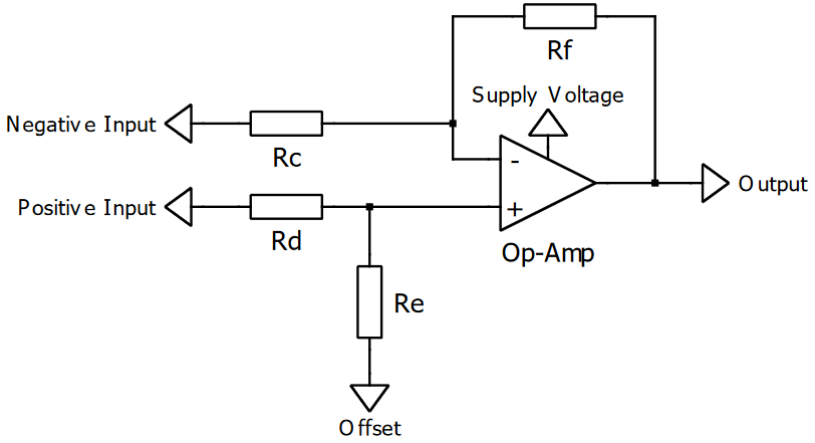
\includegraphics[scale=0.5]{hw-amplifier.png}
	\caption{Differential amplifier.}
	\label{fig:amplifier}
\end{figure}

\begin{figure}[!ht]
	\centering
	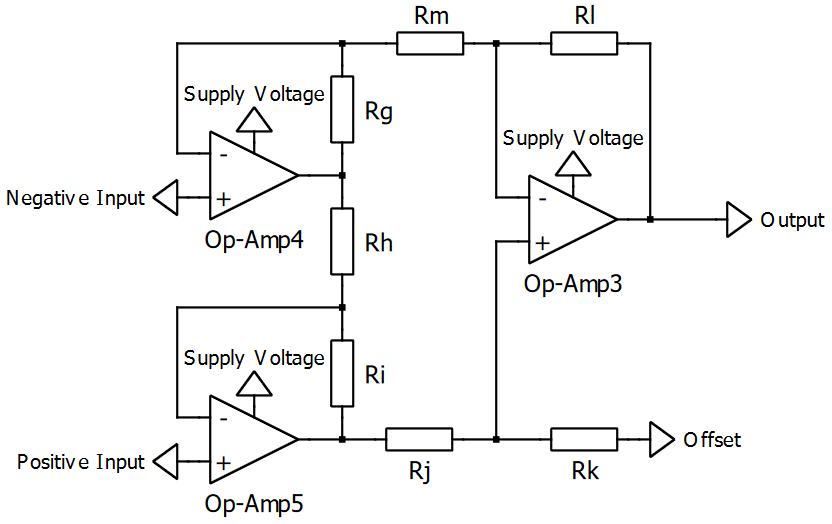
\includegraphics[scale=0.5]{hw-amplifier-1.png}
	\caption{Instrumentation amplifier.}
	\label{fig:amplifier-2}
\end{figure}

\begin{figure}[!ht]
	\centering
	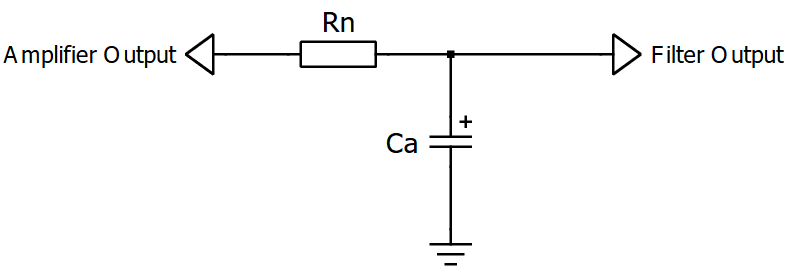
\includegraphics[scale=0.5]{hw-filter.png}
	\caption{RC lowpass filter.}
	\label{fig:filter}
\end{figure}